

%-------------------------------------------------------------------------------
% Dokumenten Klasse
\documentclass[
	final,
	a4paper,
	oneside,
	parskip=full,
	headings=standardclasses,
	headings=big,
	pointednumbers
]{scrartcl}

%-------------------------------------------------------------------------------
% Packete nutzen
\usepackage[T1]{fontenc}
\usepackage[utf8]{inputenc}
\usepackage[left=15mm,right=20mm,top=17mm,bottom=17mm,footskip=0.7cm]{geometry}
\usepackage{amsmath}
\usepackage{amssymb}
\usepackage{mathtools}
\usepackage{mathtools}
\usepackage{bm}

%-------------------------------------------------------------------------------
% Andere Schriftart
\usepackage{lmodern}

%-------------------------------------------------------------------------------
% xcolor
\usepackage[svgnames,table]{xcolor}

%-------------------------------------------------------------------------------
% scrlayer-scrpage
\usepackage{scrlayer-scrpage}
\pagestyle{scrheadings}
\clearpairofpagestyles

\cfoot{\pagemark}

%-------------------------------------------------------------------------------
% array
\usepackage{array}
\newcolumntype{A}[1]{>{\raggedright\let\newline\\\arraybackslash\hspace{0pt}}p{#1}}
\newcolumntype{B}[1]{>{\centering\let\newline\\\arraybackslash\hspace{0pt}}p{#1}}
\newcolumntype{C}[1]{>{\raggedleft\let\newline\\\arraybackslash\hspace{0pt}}p{#1}}

\newcolumntype{D}[1]{>{\raggedright\let\newline\\\arraybackslash\hspace{0pt}}m{#1}}
\newcolumntype{E}[1]{>{\centering\let\newline\\\arraybackslash\hspace{0pt}}m{#1}}
\newcolumntype{F}[1]{>{\raggedleft\let\newline\\\arraybackslash\hspace{0pt}}m{#1}}

\newcolumntype{G}[1]{>{\raggedright\let\newline\\\arraybackslash\hspace{0pt}}b{#1}}
\newcolumntype{H}[1]{>{\centering\let\newline\\\arraybackslash\hspace{0pt}}b{#1}}
\newcolumntype{I}[1]{>{\raggedleft\let\newline\\\arraybackslash\hspace{0pt}}b{#1}}


%-------------------------------------------------------------------------------
% tabularx
\usepackage{tabularx}
\usepackage{ltablex}
\usepackage{makecell}

%-------------------------------------------------------------------------------
% TikZ
\usepackage{tikz}
\usetikzlibrary{shapes, positioning, arrows, decorations, calc, fit, intersections}

%-------------------------------------------------------------------------------
% Listings
\usepackage{listings}
\newcommand{\listingMatlab}[2][]{
	\lstset{
		language=Matlab,
		breaklines=true,
		numbers=left,
		numberstyle=\tiny,
		numbersep=5pt,
		captionpos=b,
		basicstyle=\footnotesize\ttfamily,
		stringstyle=\color{magenta},
		identifierstyle=\color{black},
		keywordstyle=\color{blue}, 
		commentstyle=\color{DarkGreen}
	}
	\lstinputlisting[caption={\texttt{\detokenize{#2}}},#1]{#2}
}
\lstnewenvironment{algorithm}[1][] %defines the algorithm listing environment
{
    \lstset{ %this is the stype
        mathescape=true,
        frame=tB,
        numbers=left, 
        numberstyle=\tiny,
        basicstyle=\scriptsize, 
        keywordstyle=\color{black}\bfseries,
        keywords={,input, output, return, datatype, function, in, if, else, foreach, while, begin, end, } 
        numbers=left,
        xleftmargin=.04\textwidth
    }
}
{}


%-------------------------------------------------------------------------------

\RedeclareSectionCommand[
  afterindent=false,
  beforeskip=0.8\baselineskip,
  afterskip=0.4\baselineskip]{section}
\RedeclareSectionCommand[
  afterindent=false,
  beforeskip=0.8\baselineskip,
  afterskip=0.4\baselineskip]{subsection}

%-------------------------------------------------------------------------------
% 

\newcommand{\colouredcircle}{%
    \tikz{
        \useasboundingbox (-0.2em,-0.32em) rectangle(0.2em,0.32em);
        \draw[line width=0.03em] (0,0) circle(0.10em);
    }}



%-------------------------------------------------------------------------------
% enumitem
\usepackage{enumitem}
\newlist{tabenum}{enumerate}{3}
\setlist[tabenum,1]{
    leftmargin=*,
    label=\protect\colouredcircle,
    topsep=0ex,
    partopsep=0ex,
    noitemsep
}
\setlist[tabenum,2]{
    leftmargin=*,
    label=\protect\colouredcircle,
    topsep=0ex,
    partopsep=0ex,
    noitemsep
}
\setlist[tabenum,3]{
    leftmargin=*,
    label=\protect\colouredcircle,
    topsep=0ex,
    partopsep=0ex,
    noitemsep
}

\newcommand{\f}[2]{\frac{#1}{#2}}
\newcommand{\fs}[2]{{\tfrac{#1}{#2}}}

% kl = ()
\newcommand{\kl}[1]{{\left( #1 \right)}}

% kq = {}
\newcommand{\kq}[1]{{\left\{ #1 \right\}}}

% ks = []
\newcommand{\ks}[1]{{\left[ #1 \right]}}

% 
\newcommand{\abs}[1]{{\vert #1 \vert}}


\newcommand{\txb}[1]{{\color{blue}#1}}
\newcommand{\txr}[1]{{\color{red}#1}}
\newcommand{\txo}[1]{{\color{orange}#1}}
\newcommand{\txgr}[1]{{\color{grey}#1}}
\newcommand{\tb}[1]{\textbf{#1}}
\newcommand{\ti}[1]{\textit{#1}}

\newcommand{\tc}[1]{\multicolumn{1}{r|}{#1}}

%-------------------------------------------------------------------------------
% 
\usepackage{xparse}
% 1: Subscription  (default: '')
% 2: Funktion Name (default: 'f')
% 3: Argument      (default: 'x')
% \fx         = f(x)
% \fx[1]      = f_1(x)
% \fx[][u]    = u(x)
% \fx[][u][x] = u(x)
% \fx[][f][u] = f(u)
\NewDocumentCommand{\fx}{ O{} O{f} O{x} }{{#2_{#1}{\left( #3 \right)}}}
\NewDocumentCommand{\dfx}{ O{} O{f} O{x} }{{#2'_{#1}{\left( #3 \right)}}}
\NewDocumentCommand{\dx}{ O{} }{{\Delta x^{#1}}}
\NewDocumentCommand{\dy}{ O{} }{{\Delta y^{#1}}}
\NewDocumentCommand{\dt}{ O{} }{{\Delta t^{#1}}}
\NewDocumentCommand{\du}{ O{} }{{\Delta u^{#1}}}
\NewDocumentCommand{\px}{ O{} }{{\partial x^{#1}}}
\NewDocumentCommand{\py}{ O{} }{{\partial y^{#1}}}
\NewDocumentCommand{\pt}{ O{} }{{\partial t^{#1}}}
\NewDocumentCommand{\pu}{ O{} }{{\partial u^{#1}}}
\NewDocumentCommand{\p}{ O{} }{{\partial^{#1}}}
\NewDocumentCommand{\re}{ O{} }{{\mathbb{R}^{#1}}}

\NewDocumentCommand{\xyz}{ O{x} O{y} O{z} }{#1 #2 #3}
% 1: Value
% 2: Key
% 3: Background Color
\NewDocumentCommand{\tfill}{ O{} O{} O{blue!20} }{%
    \tikz[baseline, every node/.style={inner sep=3pt,outer sep=0pt,minimum width=3mm,minimum height=4mm}]{
        \node[fill=#3,anchor=base] (#2) {#1};
    }
}
\NewDocumentCommand{\tfillc}{ O{} O{} }{%
    \tikz[baseline, every node/.style={inner sep=2pt,outer sep=0pt}]{
        \node[fill=#2,anchor=base] {#1};
    }
}

\NewDocumentCommand{\tdrawc}{ O{} O{} }{%
    \tikz[baseline, every node/.style={inner sep=2pt,outer sep=0pt}]{
        \node[rectangle,draw=#2,anchor=base] {#1};
    }
}

\NewDocumentCommand{\tcrossc}{ O{} O{} }{%
    \tikz[baseline, every node/.style={inner sep=0pt,outer sep=0pt}]{
        \node[draw=#2,anchor=base,cross out,line width=1pt] {#1};
    }
}

\newcommand{\tfillb}[1]{\tfillc[#1][blue!20]}
\newcommand{\tfillo}[1]{\tfillc[#1][orange!40]}
\newcommand{\tfillg}[1]{\tfillc[#1][Green!20]}
\newcommand{\tfilly}[1]{\tfillc[#1][yellow!40]}
\newcommand{\tfillr}[1]{\tfillc[#1][red!20]}
\newcommand{\tfillv}[1]{\tfillc[#1][Violet!20]}
\newcommand{\tfillt}[1]{\tfillc[#1][Turquoise!20]}
\newcommand{\tfillgr}[1]{\tfillc[#1][Gray!20]}


\newcommand{\tdrawb}[1]{\tdrawc[#1][blue!40]}
\newcommand{\tdrawo}[1]{\tdrawc[#1][orange!60]}
\newcommand{\tdrawg}[1]{\tdrawc[#1][Green!40]}
\newcommand{\tdrawy}[1]{\tdrawc[#1][yellow!60]}
\newcommand{\tdrawr}[1]{\tdrawc[#1][red!40]}
\newcommand{\tdrawv}[1]{\tdrawc[#1][Violet!40]}
\newcommand{\tdrawt}[1]{\tdrawc[#1][Turquoise!40]}
\newcommand{\tdrawgr}[1]{\tdrawc[#1][Gray!40]}
\newcommand{\tdrawk}[1]{\tdrawc[#1][black]}


\newcommand{\tcrossr}[1]{\tcrossc[#1][red]}
\newcommand{\tcrossg}[1]{\tcrossc[#1][green]}
\newcommand{\tcrossb}[1]{\tcrossc[#1][blue]}

\begin{document}
    \section*{StatQuest: Logistic Regression}

    If you can fit a line...

    \begin{center}
        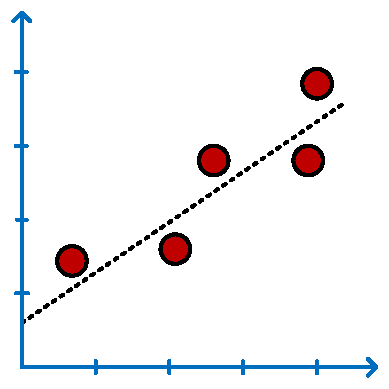
\includegraphics[height=5cm]{StatQuest_Logistic_Regression_Linear.pdf}
    \end{center}

    ... you can fit a squiggle!

    \begin{center}
        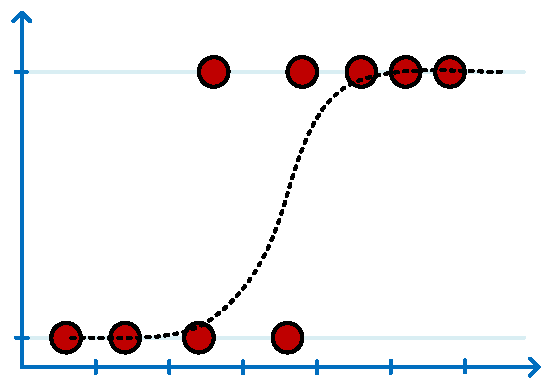
\includegraphics[height=5cm]{StatQuest_Logistic_Regression_Logistic.pdf}
    \end{center}

     Before we dive into logistic regression, let's take a step back and review linear regression.

    In another StatQuest, we talked about linear regression...  

    \begin{center}
        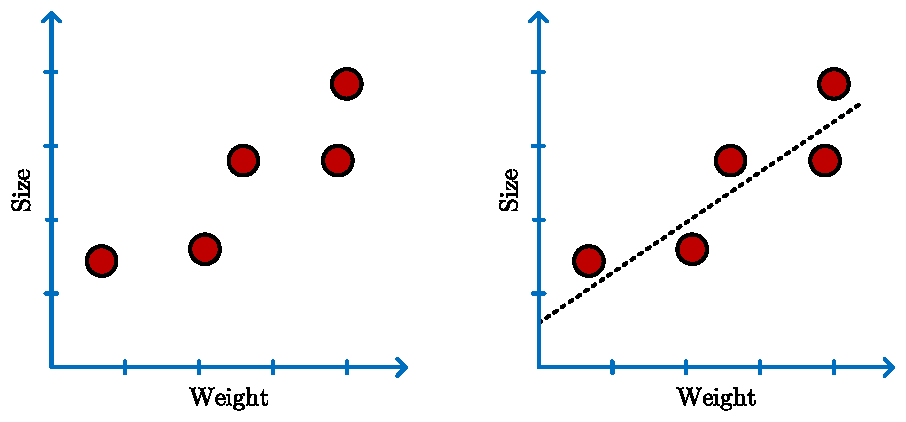
\includegraphics[height=5cm]{StatQuest_Logistic_Regression_Weight_Size.pdf}
    \end{center}

    We had some data... Then we fit a line to it... and with that line we could do a lot of things:
    \begin{enumerate}[label=\arabic*)]
        \item{
            Calculate $\bm{R^2}$ and determine if \tb{weight} and \tb{size} are correlated.
            Large values imply a large effect.
        }
        \item{
            Calculate a \tb{p-value} to determine if the $\bm{R^2}$ value is
            statistically significant.
        }
        \item{
            Use the line to predict \tb{size} given \tb{weight}.
        }
    \end{enumerate}
    
    \newpage
    
    If a new mouse has this weight... then this is the size that we predict from the weight.

    \begin{center}
        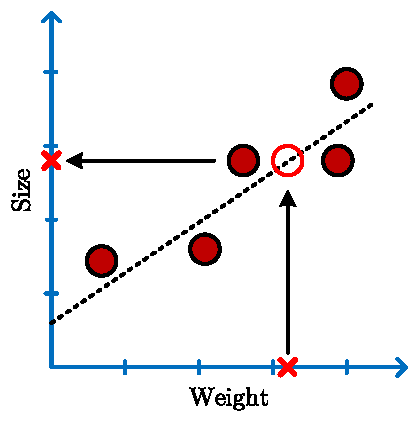
\includegraphics[height=5cm]{StatQuest_Logistic_Regression_Mouse_Weight.pdf}
    \end{center}


    Although we didn't mention it at the time, using data to predict something falls under the
    category of ``machine learning''.

    So plain old linear regression is a form of machine learning.

    We also talked a little bit about multiple regression...

    \begin{center}
        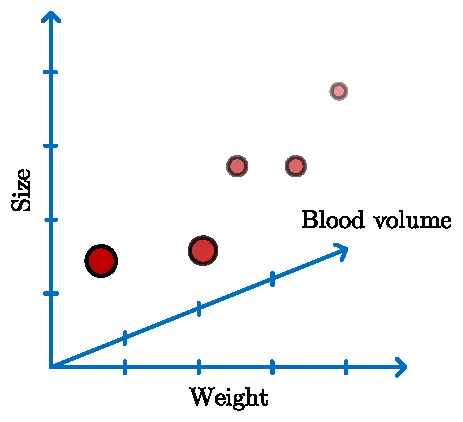
\includegraphics[height=5cm]{StatQuest_Logistic_Regression_Weight_Size_Blood.pdf}
    \end{center}

    Now we are trying to \ti{predict} \tb{size} using \tb{weight} and \tb{blood volume}.

    Alternatively, we could say we are trying to \ti{model} \tb{size} using \tb{weight} and \tb{blood volume}.

    \ti{Multiple} regression did the same things that \ti{normal} regression did...
    \begin{enumerate}[label=\arabic*)]
        \item{
            Calculate $\bm{R^2}$.
        }
        \item{
            Calculate a \tb{p-value}.
        }
        \item{
            Predict \tb{size} given \tb{weight} and \tb{blood volume}.
        }
    \end{enumerate}
    ... this is slightly fancier machine learning...

    \newpage

    We also talked about how we can use discrete measurements, like
    \tb{genotype}, to predict \tb{size}.

    \begin{center}
        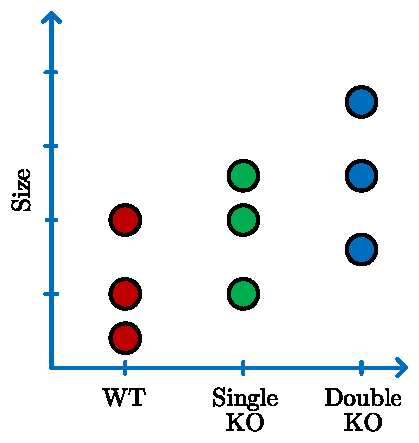
\includegraphics[height=5cm]{StatQuest_Logistic_Regression_Genotype.pdf}
    \end{center}

    If you are not familiar with the term \tb{genotype}, don't freak out.
    It's no big deal. Just know that refers to different types of mice.

    Lastly, we could compare ``models''...

    \begin{minipage}{0.40\textwidth}
        \begin{center}
            Normal regression, using \tb{weight} to predict \tb{size}.
        \end{center}
    \end{minipage}
    \begin{minipage}{0.20\textwidth}
        \begin{center}
            \tb{\LARGE vs}
        \end{center}
    \end{minipage}
    \begin{minipage}{0.40\textwidth}
        \begin{center}
            Multiple regression, using \tb{weight} and \tb{blood volume} to predict \tb{size}.
        \end{center}
    \end{minipage}

    \begin{center}
        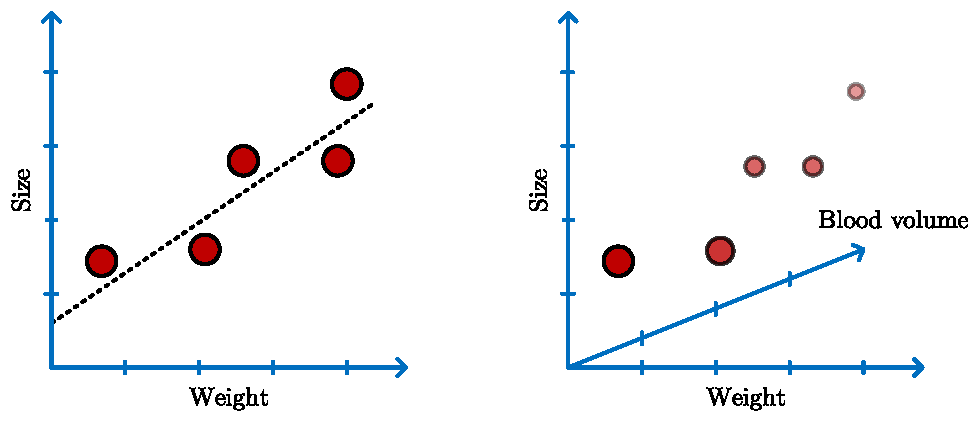
\includegraphics[height=5cm]{StatQuest_Logistic_Regression_Normal_vs_Multiple.pdf}
    \end{center}

    Comparing the \ti{simple model} to the \ti{complicated one} tells us if we need
    to measure \tb{weight} and \tb{blood volume} to accurately predict \tb{size} \ti{or}
    if we get away with just \tb{weight}.

    Now tat we remember all the cool things we can do with  \ti{linear} regression,
    lets talk about \ti{logistic} regression.

    \ti{Logistic} regression is similar to \ti{linear} regression, except...

    \begin{center}
        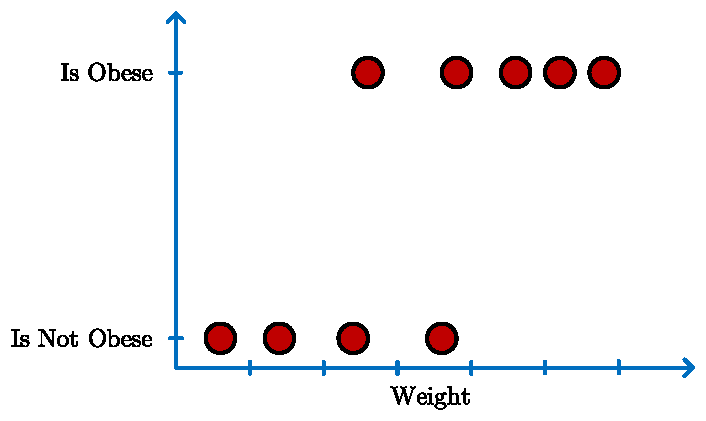
\includegraphics[height=5cm]{StatQuest_Logistic_Regression_Logistic_Obese.pdf}
    \end{center}
    
    \ti{Logistic} regression predicts whether something is \tb{True} or \tb{False}, instead
    of something \tb{continuous} like \tb{size}.

    These mice are obese... and these mice are not... also, instead of fitting a line to the data,
    logistic regression fits an ``S'' shaped ``logistic function''.

    The curve goes from 0 to 1... and that means that the curve tells you the \ti{probability}
    that a mouse is \tb{obese} based on its \tb{weight}.

    \begin{center}
        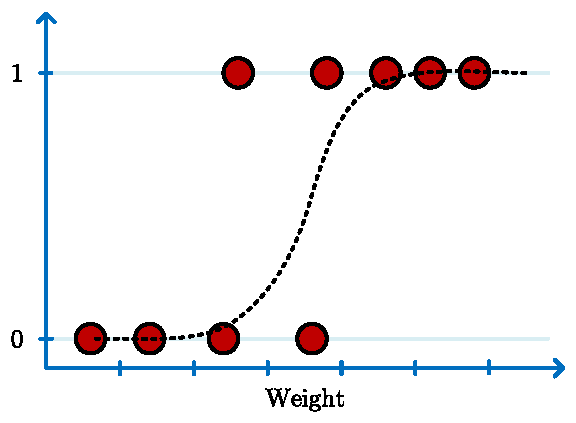
\includegraphics[height=5cm]{StatQuest_Logistic_Regression_Logistic_Boolean.pdf}
    \end{center}

    If we weighed a very heavy mouse... there is a high probability that the new mouse is obese.

    If we weighted an intermediate mouse... then there is only a $50\%$ chance that the mouse is obese.

    Lastly, there's only a small probability that a light mouse is obese.

    \begin{center}
        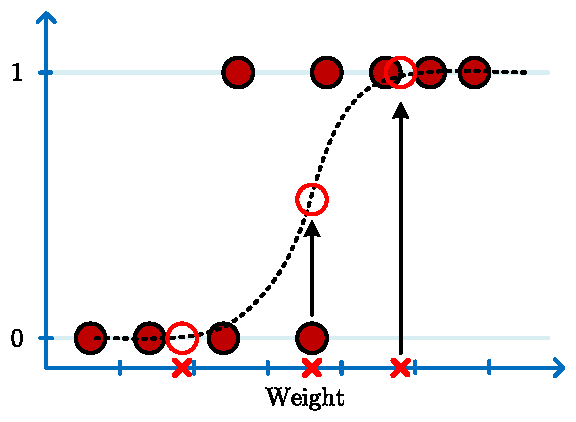
\includegraphics[height=5cm]{StatQuest_Logistic_Regression_Logistic_Percentage.pdf}
    \end{center}

    Although logistic regression tells the probability that a mouse is obese or not,
    it's usually used for \ti{classification}.

    For example, if the probability a mouse is obese is $> 50\%$, then we'll classify
    it as ``obese'', otherwise we'll classify if as ``not obese''.

    Just like with \ti{linear} regression, we can make simple models:\\
    \tb{Obesity} is predicted by \tb{Weight}

    Or more complicated models: \\
    \tb{Obesity} is predicted by \tb{Weight + Genotype} \\
    \tb{Obesity} is predicted by \tb{Weight + Genotype + Age} \\
    \tb{Obesity} is predicted by \tb{Weight + Genotype + Age + Astrological Sign}

    In other words, just like \ti{linear} regression, \ti{logistic} regression can work
    with \ti{continuous} data (like \tb{weight} and \tb{age}) and \ti{discrete} data
    (like \tb{genotype} and \tb{astrological sign}).

    We can also test to see if each variable is useful for predicting \tb{obesity}.

    However, unlike \ti{normal} regression, we can't easily compare the \ti{complicated}
    model to the \ti{simple} model (and we'll talk more about why in a bit).
    Instead, we just test to see if a variable's effect on the prediction is
    significantly different from 0. If not, it means the variable is not helping the
    prediction. We use ``Wald's Test'' to figure this out. We'll talk about that in another
    StatQuest.

    The \tb{Astrological Sign} is totally useless:\\
    \tb{Obesity} is predicted by \tb{Weight + Genotype + Age + \tcrossr{Astrological Sign}}

    That's statistical jargon or ``not helping''. That means we can save time and space
    in our study by leaving it out.

    Logistic regression's ability to provide probabilities and classify new samples using
    \ti{continuous} and \ti{discrete} measurements makes it a popular machine learning method.

    On big difference between \ti{linear} regression and \ti{logistic} regression is how the
    line is fit to the data. With \ti{linear} regression, we fit the line using ``least squares''.

    \begin{center}
        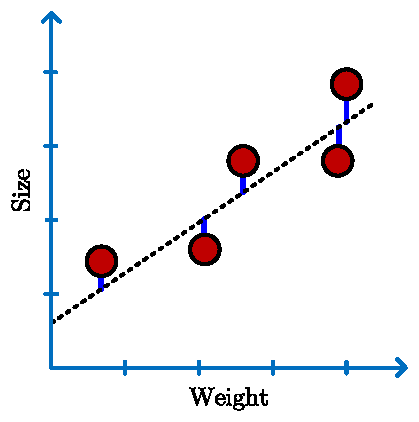
\includegraphics[height=5cm]{StatQuest_Logistic_Regression_Linear_Least_Squares.pdf}
    \end{center}

    In other words, we find the line that \tb{minimizes} the sum of the squares of
    these residuals. We also use the residuals to calculate $\bm{R^2}$ and to
    compare \ti{simple} models to \ti{complicated} models.

    Logistic regression doesn't have the same concept of a ``residual'', so it can't use
    least squares and it can't calculate $\bm{R^2}$. Instead it uses something called
    ``maximum likelihood''.

    \begin{center}
        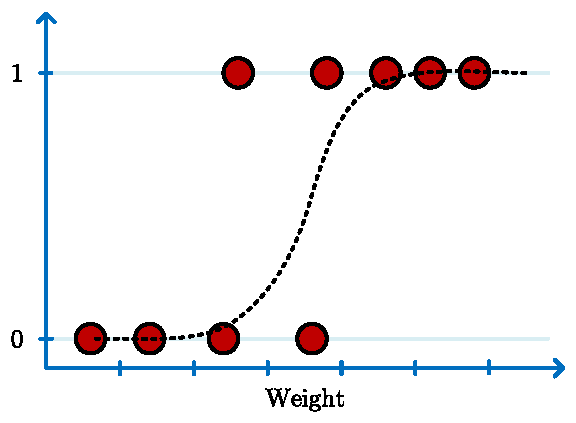
\includegraphics[height=5cm]{StatQuest_Logistic_Regression_Logistic_Boolean.pdf}
    \end{center}

    There's a whole StatQuest on maximum likelihood (so see that for details),
    but in a nutshell: You pick a probability, scaled by weight, of observing an obese mouse - just like
    this curve - and you use that to calculate the likelihood of observing a non-obese mouse that
    weighs this much, for example the first mouse. And then you calculate the likelihood of observing the
    second mouse. And you do that for all of the mice. And lastly you multiply all of those likelihoods
    together. That's the likelihood of the data given this line.

    \begin{center}
        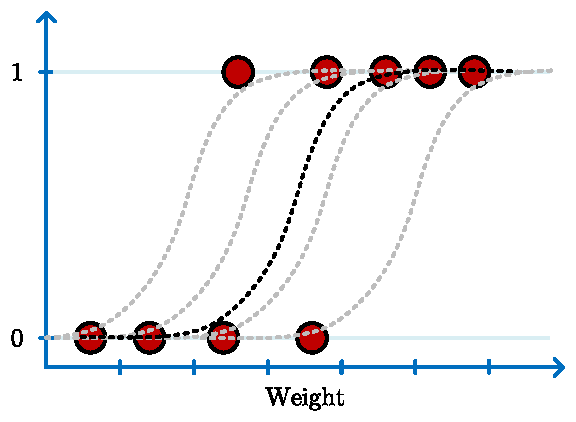
\includegraphics[height=5cm]{StatQuest_Logistic_Regression_MaxLikeli.pdf}
    \end{center}

    Then you shift the line and calculate a new likelihood of the data, then shift the line
    and calculate the likelihood again, and again. Finally, the curve with the maximum likelihood
    is selected.

    In summary: logistic regression can be used to classify samples and it can use different
    types of data (like \tb{size} and/or \tb{genotype}) to do that classification. And it
    can also be used to asses what variables are useful for classifying samples, i.e.
    \tb{astrological sign} is totally useless:

    \tb{Obesity} is predicted by \tb{Weight + Genotype + Age + \tcrossr{Astrological Sign}}

\end{document}